\newthought{\textbf{Taravia Fauzah- 2020903430054 - TRKJ 3B}}

\newday{\textbf{1 - 2 Desember 2022} - Instalasi dan Konfigurasi Hadoop}
\begin{enumerate}
\item Kendala dan Solusi
% jelaskan kendala dan penyebab yang dialami saat mengikuti praktikum serta solusi atau langkah-langkah yang telah dilakukan
\newline praktikum pertama yaitu instalasi apache hadoop. selama mengerjakan praktikum mengikuti modul tidak ada kendala

\begin{figure}[!ht]
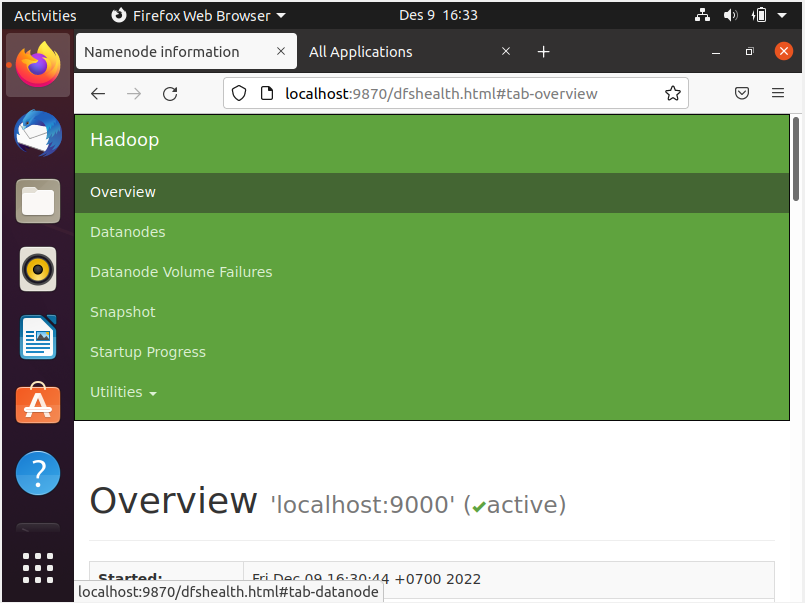
\includegraphics[width=\textwidth]{TaraviaFauzah/akses-localhost-9078}
\caption{hasil dari cek hadoop service}
\label{gam:perkuliahan15-9}
\end{figure}

\begin{figure}[!ht]
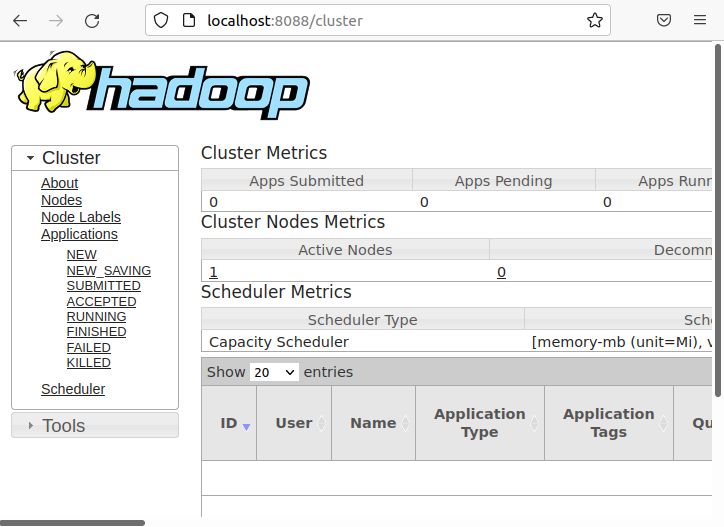
\includegraphics[width=\textwidth]{TaraviaFauzah/akses-localhost-8088}
\caption{hasil dari cek hadoop service}
\label{gam:perkuliahan15-9}
\end{figure}

\item Kesimpulan
% berikan kesimpulan dari praktikum yang telah dikerjkan
\newline Berhasil mendownload dan menginstal Apache hadoop dan sudah bisa di jalankan 
\end{enumerate}

\newday{\textbf{8 Desember 2022} - WordCount bawaan Hadoop}
\begin{enumerate}
\item Kendala dan Solusi
% jelaskan kendala dan penyebab yang dialami saat mengikuti praktikum serta solusi atau langkah-langkah yang telah dilakukan
\newline pada praktikum kali ini membuat program WordCount Bawaan Hadoop.pada saat praktikum tidak ada kendala hanya saja error karena salah menulis perintah.

\begin{figure}[!ht]
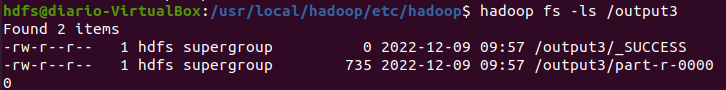
\includegraphics[width=\textwidth]{TaraviaFauzah/output}
\caption{hasil dari hadoop fs}
\label{gam:perkuliahan1-10}
\end{figure}

\begin{figure}[!ht]
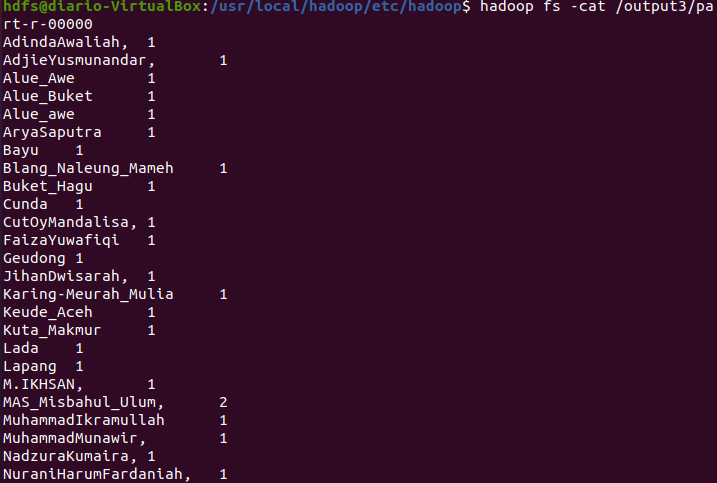
\includegraphics[width=\textwidth]{TaraviaFauzah/output1}
\caption{hasil dari hadoop fs}
\label{gam:perkuliahan1-10}
\end{figure}

\begin{figure}[!ht]
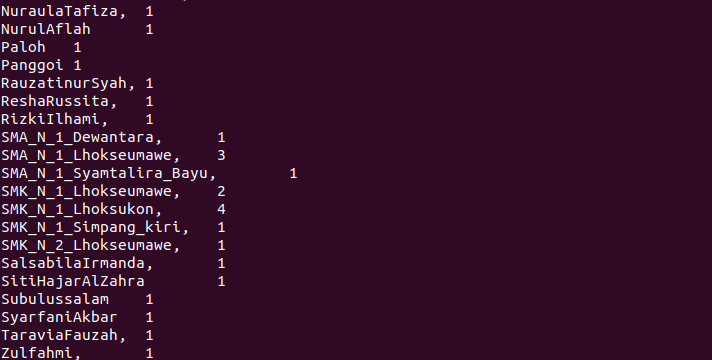
\includegraphics[width=\textwidth]{TaraviaFauzah/output1_1}
\caption{hasil dari hadoop fs}
\label{gam:perkuliahan1-10}
\end{figure}

\item Kesimpulan
% berikan kesimpulan dari praktikum yang telah dikerjkan
\newline langkah praktikum ini adalah untuk memahami proses cara kerja pada hadoop dalam memproses data input sehingga menghasikan sebuah output. wordcount adalah program untuk menghitung jumlah kata dalam inpu.

\end{enumerate}

\newday{\textbf{9 Desember 2022} - WordCount dengan Java}
\begin{enumerate}
\item Kendala dan Solusi
% jelaskan kendala dan penyebab yang dialami saat mengikuti praktikum serta solusi atau langkah-langkah yang telah dilakukan
\newline pada praktikum kali ini membuat program WordCount dengan java.pada saat praktikum memiliki error tapi errornya di sebabkan tidak teliti saat menulis codingan yang ada di modul.solusinya harus lebih teliti saat mengerjakan codingan tersebut.

\begin{figure}[!ht]
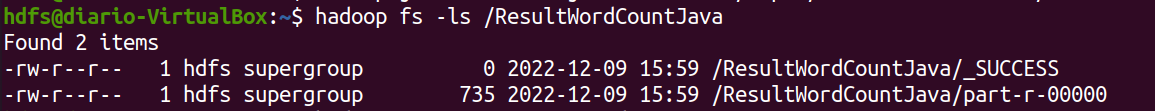
\includegraphics[width=\textwidth]{TaraviaFauzah/hasil1}
\caption{hasil dari hadoop fs WordCount}
\label{gam:perkuliahan2-12}
\end{figure}

\begin{figure}[!ht]
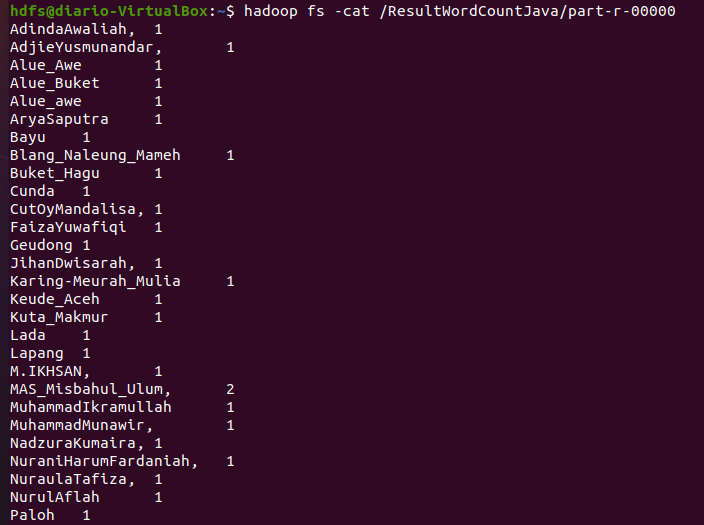
\includegraphics[width=\textwidth]{TaraviaFauzah/hasil2}
\caption{hasil dari hadoop fs WordCount}
\label{gam:perkuliahan2-12}
\end{figure}

\begin{figure}[!ht]
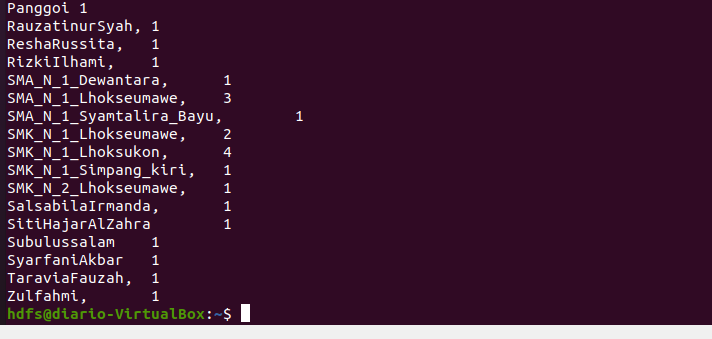
\includegraphics[width=\textwidth]{TaraviaFauzah/hasil2_2}
\caption{hasil dari hadoop fs WordCount}
\label{gam:perkuliahan2-12}
\end{figure}

\item Kesimpulan
% berikan kesimpulan dari praktikum yang telah dikerjkan
\newline berhasil menjalan program WordCount dengan java

\end{enumerate}

\newday{\textbf{15 Desember 2022}}
\begin{enumerate}
\item Kendala dan Solusi
% jelaskan kendala dan penyebab yang dialami saat mengikuti praktikum serta solusi atau langkah-langkah yang telah dilakukan
\newline pada praktikum kali ini instalasi apache spark (pyspark)tidak ada kendala.

\begin{figure}[!ht]
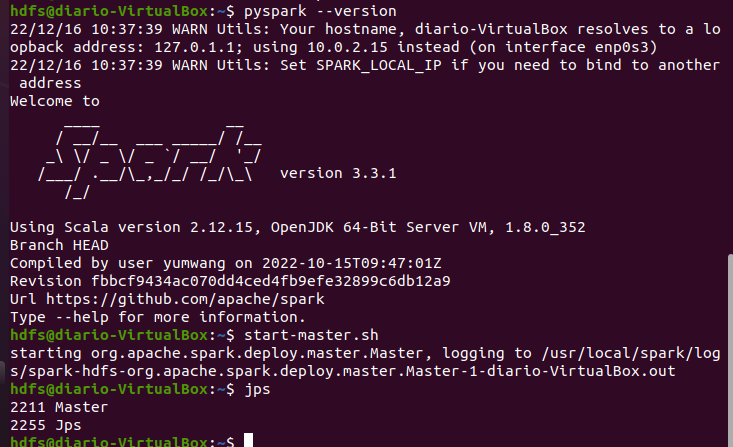
\includegraphics[width=\textwidth]{TaraviaFauzah/pyspark version}
\caption{hasil dari pyspark version}
\label{gam:perkuliahan2-15}
\end{figure}

\item Kesimpulan
% berikan kesimpulan dari praktikum yang telah dikerjkan
\newline berhasil menjalan pyspark yang sudah terinstall.
\end{enumerate}

\newday{\textbf{16 Desember 2022}}
\begin{enumerate}
\item Kendala dan Solusi
% jelaskan kendala dan penyebab yang dialami saat mengikuti praktikum serta solusi atau langkah-langkah yang telah dilakukan

\item Kesimpulan
% berikan kesimpulan dari praktikum yang telah dikerjkan

\end{enumerate}

\newday{\textbf{22 Desember 2022}}
\begin{enumerate}
\item Kendala dan Solusi
% jelaskan kendala dan penyebab yang dialami saat mengikuti praktikum serta solusi atau langkah-langkah yang telah dilakukan

\item Kesimpulan
% berikan kesimpulan dari praktikum yang telah dikerjkan

\end{enumerate}